\documentclass[main.tex]{subfiles}
\begin{document}
至二十世纪之前,人们对液态体系的理论认识十分有限。关于液态,大家的理解程度仅限于范德华方程。以至溶液,也仅知道拉乌尔定律和范托夫定律。显然,实际体系常常偏离这些简单定理。因此,探寻溶液的非理想现象(例如相对拉乌尔定律的偏离)的化学或微观根源,很快就成为了研究的主题\cite{Hildebrand1981}。经过将近二十年的争论,大家渐渐接受了分子间相互作用势在混合前后的差异是溶液行为偏离理想行为的原因。1916年,J. Hildebrand在前人的基础上总结了溶液非理想性与分子间相互作用势的关系\cite{Hildebrand1916},也就是溶液的分子间相互作用势与各组分纯物质的分子间相互作用势的\emph{差别}导致了溶液的非理想性。这个物理图像被承认至今。

作为背景,在这里提一下在当时同样正在形成的混合物热力学和统计力学理论体系。在1901\textasciitilde 1910年期间,G. Lewis陆续提出了现在见于主流热力学教材的“偏摩尔量”、“逸度”、“活度”的概念体系\cite{Lewis1901,Lewis1907},为描述一般真实混合物提供了完善而且数学表达简洁的概念体系。但这个体系在当时并未迅速获得像在今天这样的广泛统治性地位。在当时统计力学刚刚开始被用于解决实际问题。R. Fowler是统计力学除J. Gibbs、之外的另一位奠基人。尽管吉布斯在1902年出版的里程碑式著作\emph{Elementary Principles in Statistical Mechanics}\cite{Gibbs1902}中几乎以现代形式奠定了统计力学的系综方法,但其对当时日常热力学计算的推广相对缓慢。直至在英国的Fowler在1929年出版的统计力学教材\cite{Fowler1929}推动了以配分函数为核心的精确热力学性质计算在教学与研究中的普及。随后,Fowler与他第一名学生E. Guggenheim合著的统计热力学(首版于1939)\cite{Fowler1939}进一步系统化了这一途径,并在物理与化学界确立为常规方法。

回到溶液理论的历史。1920\textasciitilde 1929年期间,Hildebrand发表了一系列论文,提出“正规溶液”的概念\cite{Hildebrand1951},即超额混合熵变为零的溶液(因而它允许混合焓变不为零)。这是一种比理想溶液适用范围更广的参考体系。正规溶液的提出,一方面把人们的注意力集中到了非零混合焓变的微观机理的研究上,另一方面也突出了超额熵不为零之微观原因这一理论空白。正规溶液在合金材料领域立刻得到了响应,因为正规溶液的混合自由能可以解释合金材料当中的有序无序转变。Bragg和Williams\cite{Bragg1934,Bragg1935}正是在合金的研究兴趣背景下提出以他们命名的平均场近似的。

至此,人们普遍认为只要$\Delta_\text{mix}H= 0$,溶液就是理想的。1935年,Guggenheim首次注意到\cite{Guggenheim1935},这一结论还需加上“溶质与溶剂分子尺寸相近”的必要条件。这个结论是他在通过统计力学推导出理想溶液混合熵的过程中发现的。也正是在这个推导任务中,Guggenheim使用了格子模型。这应该是格子模型在溶液热力学中的首次使用。

Bragg--Wiilliams平均场近似的结果与实验的差异,继续引起当时研究者的关注。1935年H.Bethe首次认识到,既然假定了分子间作用势的差异,就不能再假定分子间完全随机混匀\cite{Bethe1935}。他在这篇论文中首次提出一种方法去考虑有序相邻对的条件概率。按照Bethe的方法,可以按需考虑任一中心格子之外数层分子的种类的条件概率。但实际操作下,到第二层已经十分繁琐,因此第一层的结果——也就是有序相邻对的条件概率——获得了重视。次年,R. Peierls重新梳理了Bethe的方法,提出了一种通过自洽性原则来处理有序相邻对的条件概率的方法\cite{Peierls1936},使得数学操作从人工枚举转化为积分微分方程。这个近似今天也被称为Bethe--Peierls近似。至此,这些研究工作都是以合金材料为研究背景的。

另一方面,Fowler不断尝试用他当时建立的统计力学基本理论来处理各种实际问题。其中他采用格子模型来处理气体在固体表面吸附的问题\cite{Fowler1936},这个问题在数学模型上跟二元混合物是相同的。Fowler在这篇论文里仍然只做了平均场假定。Peierls认识Bethe的方法也可以用到这个实际问题中\cite{Peierls1936a}。他的论文发表后,Fowler的另一名学生——中国科学家张宗燧——就接着进行Bethe--Peierls方法的推广和一般化的数学物理工作,发表了一系列论文\cite{Chang1938,Chang1939},最终在1939年已赴哥本哈根后发表了最具一般性的结果:把$n$个球放入$N>n$个格子中,使得连续两格都有球的总数为$X$的方法数$g_2\left(N,n,X\right)$的表达式\cite{Chang1939b}。其中,Fowler的又一名中国学生——王竹溪,也在期间发表了相关的工作\cite{Wang1937}。王竹溪回国后在西南联大任教。杨振宁在王竹溪的指导下攻读硕士期间继续了关于溶液格子模型统计的工作\cite{Yang1983}。1945年,他针对Bethe--Peierls方法的计算需要计算一个很难的微分积分方程的问题,提出了一个勒让德变换的聪明技巧,不仅解决了Bethe的一阶近似,还可以推广到比最邻近相互作用更加远程的相关性的计算\cite{Yang1945}。在此基础上,1949年李荫远发表了在不同实际体系上的应用工作\cite{Li1949}。可以说,中国科学家在那个尽管艰苦的年代,在溶液格子模型统计的研究领域仍洒下了浓墨重彩的一笔。

以上工作均把重点放在了非零的相互作用势如何影响分子排布的局域相关性,从而影响混合熵变上,一般是假定溶剂和溶质分子尺寸相当的,因而属于相对于正规溶液的偏离。自1935年Guggenheim提出尺寸相当是$\Delta_\text{mix}H=0$时溶液为理想溶液的必要条件后,他在1936年的会议上再次强调这一点\cite{Guggenheim1937}并引起了更广泛的重视。1937年Fowler和Rushbrooke首先尝试了溶质为2聚体(占两个格子)的推导\cite{Fowler1937}。在当时,无论是混合熵还是混合焓都是需要写下配分函数后给出的,后者需要计数构形数。Fowler和Rushbrooke在这篇论文中没有采用Bethe的方法,仅得出$N_1\ll N_2$和$N_1\gg N_2$的情况,至少证明了哪怕$\Delta_\text{mix}H=0$, 仅由于溶质尺寸较大,也会使溶液偏离拉乌尔定律。准确的二聚体结果则由张宗燧于1939年给出\cite{Chang1939a}。A. Miller于1942年推广到了三聚体的情况\cite{Miller1942,Miller1943}。1944年W. Orr用Bethe方法给出了一般$r$聚体的结果\cite{Orr1944}。

同在1944年Guggenheim为这件本已划上句号的事情作了实质上更重要的贡献。他用比Bethe--Peierls更简单的方法得出了$r$聚体的无热混合熵,并确认了张宗燧和Miller关于二聚体和三聚体的结果\cite{Guggenheim1944};同时又证明了Bethe的一阶近似,跟他提出的准化学近似是等价的\cite{Guggenheim1944a}。精细平衡的考虑和准化学近似,都在物理上作为更充份的理由支撑了Bethe--Peierls的做法,而且数学推导大大简化至本科一年级数学的水平。这些两大成果总结在了他于1952年出版的书中\cite{Guggenheim1952},也已经体现在本讲义之前几节的讲述当中。

\begin{figure}[ht]
  \centering
  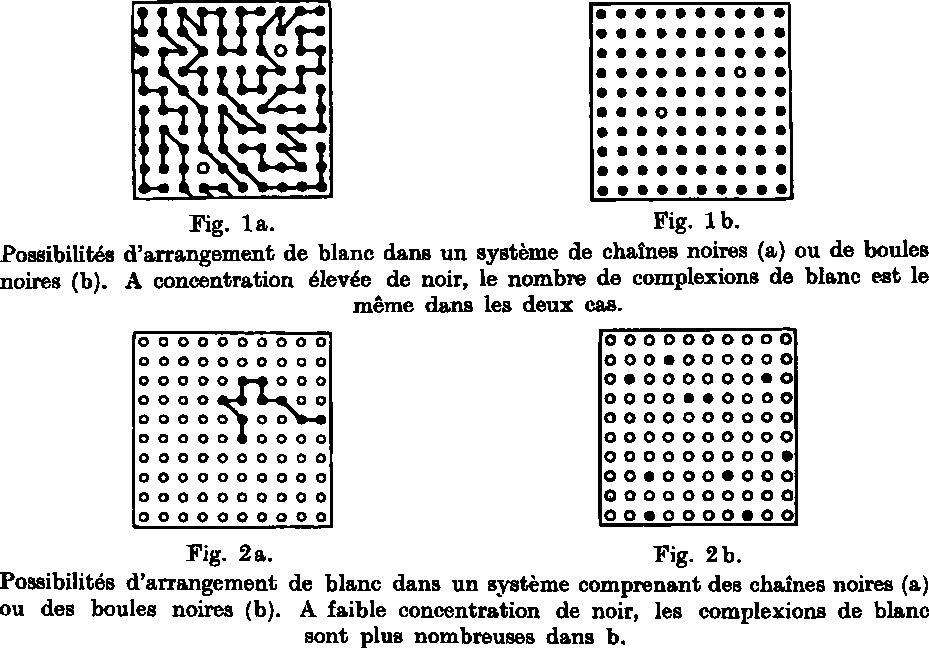
\includegraphics{../images/meyer_illustration.pdf}
  \caption{K. Meyer在1940年的论文中展示大分子与小分子溶质的构形数。Fig. 1是浓溶液情况,溶剂分子的排布方法数在大分子和小分子溶液中差不多;Fig. 2是稀溶液情况,溶剂分子的排布方法数在小分子溶液中远大于大分子溶液。Meyer认为这种差异是造成超额混合熵的原因。图自\cite{Meyer1940}。}
  \label{fig:meyer_illustration}
\end{figure}

从Bragg开始介绍的主要是发生在英国的研究进展(杨振宁的工作除外)。1935年,K. Meyer和Lühdemann发表的论文报道了几种大分子溶质(分子量几百左右)在一系列溶剂中的溶液的渗透压数据,旨在研究溶液的非理想性\cite{Meyer1935}。他们发现了所研究的体系有超额混合熵。1936年,E. Hückel\cite{Hueckel1936}推导了范托夫定律的偏离展开式,发现一次近似系数含有混合物组份分子体积的比,因此暗示了仅分子体积差异就足以造成非理想性。他在同一篇论文中分析了Meyer和Lühdemann的实验数据,发现数据支持了这一说法。1937年法国科学家C. Boissonnas用量热法直接测混合焓变,同时结合已报道的混合自由能数据计算混合熵变,发现了正的超额混合熵变\cite{Boissonnas1937}。前面提到过的Fowler和Rushbrooke在1937年的工作,理论上证实了分子尺寸差异足以造成超额混合熵变,这引起了Meyer的重视。1940年Meyer对之前的实验结果进行总结\cite{Meyer1940},正式提出大分子溶质溶解增加超额混合熵的物理原因是这种分子有大量的“内部活动性”(effet de mobilité intérieure)。在这篇论文中的插图(见图\ref{fig:meyer_illustration})已十分接近今天教科书中高分子溶液格子理论的图示。

至1940年,Guggenheim、Fowler、Rushbrooke、Hückel和Meyer等人在英国和欧洲大陆的工作开始引起了在美国的M. Huggins的重视,他在1941年发表了第一篇论文\cite{Huggins1941}。根据Flory自述\cite{Flory1985},他第一次了解到Huggins的工作,是在1941年6月于康奈尔大学举行的胶体研讨会上。在那次研讨会上,Flory发表了一篇关于非线形聚合物凝胶化和网络形成理论的论文,这个主题与溶液热力学内容无关,后来也获得了广泛的认可。从Huggins的演讲中,Flory惊讶地得知他所进行的工作与Flory当时正准备发表的关于聚合物溶液热力学的研究非常相似。演讲结束后,Flory跟Huggins说他也在进行类似的研究。Huggins非常和蔼地鼓励作为他晚辈的Flory。Flory在同年稍晚于Huggins发表了他关于溶液热力学的论文\cite{Flory1941}。正如本讲义之前总结的那要,Flory--Huggins正确地得出了高分子无热溶液的混合熵变在配位数$z\to\infty$的结果,同时按平均场近似得出了混合焓变的结果。

虽然1960年以来非格子的统计力学得到了长足发展,包括聚合物溶液在内的液体统计力学中,格子模型已非主流,但它仍然在获得近世化的改善。最值得注意的是K. Freed及其同事的多年工作。Freed基于格子模型做了类似Mayer集团展开的处理。使得格子模型可作为一个不亚于非格子统计模型的液体研究手段\cite{Dudowicz1990},应用于不限于溶液,甚至不限液态聚合物体系问题中\cite{Foreman1998,Dudowicz2007,Xu2016}。格子模型对粒子空间排布的离散化处理,使得计算构形数——即粒子排布方式的总数——这件艰巨任务有可行性。在应用方面,1970年代形成的UNIQUAC(UNIversal QUAsiChemical)模型\cite{Abrams1975,Maurer1978}已成为常用的液体热力学参数计算模型,常用于相平衡(即液--固、液--液或液--气平衡)的描述。正如前面介绍的那样,准化学近似只是Bethe的一阶近似。最新的COSMOSPACE模型\cite{Klamt2002}则通过自洽原则给出了适用于更加强相关体系的应用模型。这些都说明,格子模型至今仍是液态物理理论与应用研究的重要理论模型。
\end{document}